% Options for packages loaded elsewhere
\PassOptionsToPackage{unicode}{hyperref}
\PassOptionsToPackage{hyphens}{url}
\PassOptionsToPackage{dvipsnames,svgnames,x11names}{xcolor}
%
\documentclass[
  letterpaper,
  DIV=11,
  numbers=noendperiod]{scrartcl}

\usepackage{amsmath,amssymb}
\usepackage{iftex}
\ifPDFTeX
  \usepackage[T1]{fontenc}
  \usepackage[utf8]{inputenc}
  \usepackage{textcomp} % provide euro and other symbols
\else % if luatex or xetex
  \usepackage{unicode-math}
  \defaultfontfeatures{Scale=MatchLowercase}
  \defaultfontfeatures[\rmfamily]{Ligatures=TeX,Scale=1}
\fi
\usepackage{lmodern}
\ifPDFTeX\else  
    % xetex/luatex font selection
\fi
% Use upquote if available, for straight quotes in verbatim environments
\IfFileExists{upquote.sty}{\usepackage{upquote}}{}
\IfFileExists{microtype.sty}{% use microtype if available
  \usepackage[]{microtype}
  \UseMicrotypeSet[protrusion]{basicmath} % disable protrusion for tt fonts
}{}
\makeatletter
\@ifundefined{KOMAClassName}{% if non-KOMA class
  \IfFileExists{parskip.sty}{%
    \usepackage{parskip}
  }{% else
    \setlength{\parindent}{0pt}
    \setlength{\parskip}{6pt plus 2pt minus 1pt}}
}{% if KOMA class
  \KOMAoptions{parskip=half}}
\makeatother
\usepackage{xcolor}
\setlength{\emergencystretch}{3em} % prevent overfull lines
\setcounter{secnumdepth}{-\maxdimen} % remove section numbering
% Make \paragraph and \subparagraph free-standing
\ifx\paragraph\undefined\else
  \let\oldparagraph\paragraph
  \renewcommand{\paragraph}[1]{\oldparagraph{#1}\mbox{}}
\fi
\ifx\subparagraph\undefined\else
  \let\oldsubparagraph\subparagraph
  \renewcommand{\subparagraph}[1]{\oldsubparagraph{#1}\mbox{}}
\fi

\usepackage{color}
\usepackage{fancyvrb}
\newcommand{\VerbBar}{|}
\newcommand{\VERB}{\Verb[commandchars=\\\{\}]}
\DefineVerbatimEnvironment{Highlighting}{Verbatim}{commandchars=\\\{\}}
% Add ',fontsize=\small' for more characters per line
\usepackage{framed}
\definecolor{shadecolor}{RGB}{241,243,245}
\newenvironment{Shaded}{\begin{snugshade}}{\end{snugshade}}
\newcommand{\AlertTok}[1]{\textcolor[rgb]{0.68,0.00,0.00}{#1}}
\newcommand{\AnnotationTok}[1]{\textcolor[rgb]{0.37,0.37,0.37}{#1}}
\newcommand{\AttributeTok}[1]{\textcolor[rgb]{0.40,0.45,0.13}{#1}}
\newcommand{\BaseNTok}[1]{\textcolor[rgb]{0.68,0.00,0.00}{#1}}
\newcommand{\BuiltInTok}[1]{\textcolor[rgb]{0.00,0.23,0.31}{#1}}
\newcommand{\CharTok}[1]{\textcolor[rgb]{0.13,0.47,0.30}{#1}}
\newcommand{\CommentTok}[1]{\textcolor[rgb]{0.37,0.37,0.37}{#1}}
\newcommand{\CommentVarTok}[1]{\textcolor[rgb]{0.37,0.37,0.37}{\textit{#1}}}
\newcommand{\ConstantTok}[1]{\textcolor[rgb]{0.56,0.35,0.01}{#1}}
\newcommand{\ControlFlowTok}[1]{\textcolor[rgb]{0.00,0.23,0.31}{#1}}
\newcommand{\DataTypeTok}[1]{\textcolor[rgb]{0.68,0.00,0.00}{#1}}
\newcommand{\DecValTok}[1]{\textcolor[rgb]{0.68,0.00,0.00}{#1}}
\newcommand{\DocumentationTok}[1]{\textcolor[rgb]{0.37,0.37,0.37}{\textit{#1}}}
\newcommand{\ErrorTok}[1]{\textcolor[rgb]{0.68,0.00,0.00}{#1}}
\newcommand{\ExtensionTok}[1]{\textcolor[rgb]{0.00,0.23,0.31}{#1}}
\newcommand{\FloatTok}[1]{\textcolor[rgb]{0.68,0.00,0.00}{#1}}
\newcommand{\FunctionTok}[1]{\textcolor[rgb]{0.28,0.35,0.67}{#1}}
\newcommand{\ImportTok}[1]{\textcolor[rgb]{0.00,0.46,0.62}{#1}}
\newcommand{\InformationTok}[1]{\textcolor[rgb]{0.37,0.37,0.37}{#1}}
\newcommand{\KeywordTok}[1]{\textcolor[rgb]{0.00,0.23,0.31}{#1}}
\newcommand{\NormalTok}[1]{\textcolor[rgb]{0.00,0.23,0.31}{#1}}
\newcommand{\OperatorTok}[1]{\textcolor[rgb]{0.37,0.37,0.37}{#1}}
\newcommand{\OtherTok}[1]{\textcolor[rgb]{0.00,0.23,0.31}{#1}}
\newcommand{\PreprocessorTok}[1]{\textcolor[rgb]{0.68,0.00,0.00}{#1}}
\newcommand{\RegionMarkerTok}[1]{\textcolor[rgb]{0.00,0.23,0.31}{#1}}
\newcommand{\SpecialCharTok}[1]{\textcolor[rgb]{0.37,0.37,0.37}{#1}}
\newcommand{\SpecialStringTok}[1]{\textcolor[rgb]{0.13,0.47,0.30}{#1}}
\newcommand{\StringTok}[1]{\textcolor[rgb]{0.13,0.47,0.30}{#1}}
\newcommand{\VariableTok}[1]{\textcolor[rgb]{0.07,0.07,0.07}{#1}}
\newcommand{\VerbatimStringTok}[1]{\textcolor[rgb]{0.13,0.47,0.30}{#1}}
\newcommand{\WarningTok}[1]{\textcolor[rgb]{0.37,0.37,0.37}{\textit{#1}}}

\providecommand{\tightlist}{%
  \setlength{\itemsep}{0pt}\setlength{\parskip}{0pt}}\usepackage{longtable,booktabs,array}
\usepackage{calc} % for calculating minipage widths
% Correct order of tables after \paragraph or \subparagraph
\usepackage{etoolbox}
\makeatletter
\patchcmd\longtable{\par}{\if@noskipsec\mbox{}\fi\par}{}{}
\makeatother
% Allow footnotes in longtable head/foot
\IfFileExists{footnotehyper.sty}{\usepackage{footnotehyper}}{\usepackage{footnote}}
\makesavenoteenv{longtable}
\usepackage{graphicx}
\makeatletter
\def\maxwidth{\ifdim\Gin@nat@width>\linewidth\linewidth\else\Gin@nat@width\fi}
\def\maxheight{\ifdim\Gin@nat@height>\textheight\textheight\else\Gin@nat@height\fi}
\makeatother
% Scale images if necessary, so that they will not overflow the page
% margins by default, and it is still possible to overwrite the defaults
% using explicit options in \includegraphics[width, height, ...]{}
\setkeys{Gin}{width=\maxwidth,height=\maxheight,keepaspectratio}
% Set default figure placement to htbp
\makeatletter
\def\fps@figure{htbp}
\makeatother

\KOMAoption{captions}{tableheading}
\makeatletter
\makeatother
\makeatletter
\makeatother
\makeatletter
\@ifpackageloaded{caption}{}{\usepackage{caption}}
\AtBeginDocument{%
\ifdefined\contentsname
  \renewcommand*\contentsname{Table of contents}
\else
  \newcommand\contentsname{Table of contents}
\fi
\ifdefined\listfigurename
  \renewcommand*\listfigurename{List of Figures}
\else
  \newcommand\listfigurename{List of Figures}
\fi
\ifdefined\listtablename
  \renewcommand*\listtablename{List of Tables}
\else
  \newcommand\listtablename{List of Tables}
\fi
\ifdefined\figurename
  \renewcommand*\figurename{Figure}
\else
  \newcommand\figurename{Figure}
\fi
\ifdefined\tablename
  \renewcommand*\tablename{Table}
\else
  \newcommand\tablename{Table}
\fi
}
\@ifpackageloaded{float}{}{\usepackage{float}}
\floatstyle{ruled}
\@ifundefined{c@chapter}{\newfloat{codelisting}{h}{lop}}{\newfloat{codelisting}{h}{lop}[chapter]}
\floatname{codelisting}{Listing}
\newcommand*\listoflistings{\listof{codelisting}{List of Listings}}
\makeatother
\makeatletter
\@ifpackageloaded{caption}{}{\usepackage{caption}}
\@ifpackageloaded{subcaption}{}{\usepackage{subcaption}}
\makeatother
\makeatletter
\@ifpackageloaded{tcolorbox}{}{\usepackage[skins,breakable]{tcolorbox}}
\makeatother
\makeatletter
\@ifundefined{shadecolor}{\definecolor{shadecolor}{rgb}{.97, .97, .97}}
\makeatother
\makeatletter
\makeatother
\makeatletter
\makeatother
\ifLuaTeX
  \usepackage{selnolig}  % disable illegal ligatures
\fi
\IfFileExists{bookmark.sty}{\usepackage{bookmark}}{\usepackage{hyperref}}
\IfFileExists{xurl.sty}{\usepackage{xurl}}{} % add URL line breaks if available
\urlstyle{same} % disable monospaced font for URLs
\hypersetup{
  pdftitle={Taylor Series},
  colorlinks=true,
  linkcolor={blue},
  filecolor={Maroon},
  citecolor={Blue},
  urlcolor={Blue},
  pdfcreator={LaTeX via pandoc}}

\title{Taylor Series}
\author{}
\date{}

\begin{document}
\maketitle
\ifdefined\Shaded\renewenvironment{Shaded}{\begin{tcolorbox}[sharp corners, borderline west={3pt}{0pt}{shadecolor}, enhanced, frame hidden, interior hidden, boxrule=0pt, breakable]}{\end{tcolorbox}}\fi

\begin{equation}
f(x) = \sum_{n=0}^{\infty}\frac{f^{(n)}(a)}{n!}(x-a)^{n}
\end{equation}

Let \(f(x)\) be a function that is \(n+1\) times differentiable on an
interval \(I\) containing \(a\) and let \(P_n(x)\) be the \(n\)th degree
Taylor polynomial for \(f(x)\) about \(a\). Then, there exists a number
\(c\) between \(a\) and \(x\) such that: \begin{equation}
f(x)=P_n(x)+R_n(x),
\end{equation} where the remainder \(R_n(x)\) is given by:
\begin{equation}
R_n(x)=\frac{f^{(n+1)}(c)}{(n+1)!}(x-a)^{n+1}.
\end{equation}

\hypertarget{define-the-function-to-be-approximated}{%
\section{Define the function to be
approximated}\label{define-the-function-to-be-approximated}}

\begin{Shaded}
\begin{Highlighting}[]
\ImportTok{import}\NormalTok{ torch}
\ImportTok{import}\NormalTok{ math}
\ImportTok{import}\NormalTok{ matplotlib.pyplot }\ImportTok{as}\NormalTok{ plt}
\ImportTok{import}\NormalTok{ numpy }\ImportTok{as}\NormalTok{ np}
\CommentTok{\# Define the sine function to be approximated}
\KeywordTok{def}\NormalTok{ f(x):}
    \ControlFlowTok{return}\NormalTok{ torch.sin(x)}

\NormalTok{x }\OperatorTok{=}\NormalTok{ torch.linspace(}\OperatorTok{{-}}\FloatTok{3.14}\NormalTok{, }\FloatTok{3.14}\NormalTok{, }\DecValTok{100}\NormalTok{)}
\NormalTok{y }\OperatorTok{=}\NormalTok{ f(x)}
\NormalTok{plt.plot(x, y)}
\NormalTok{plt.xlabel(}\StringTok{\textquotesingle{}x\textquotesingle{}}\NormalTok{)}
\NormalTok{plt.ylabel(}\StringTok{\textquotesingle{}y\textquotesingle{}}\NormalTok{)}
\NormalTok{plt.title(}\StringTok{\textquotesingle{}Sine Function\textquotesingle{}}\NormalTok{)}
\NormalTok{plt.show()}
\end{Highlighting}
\end{Shaded}

\begin{figure}[H]

{\centering 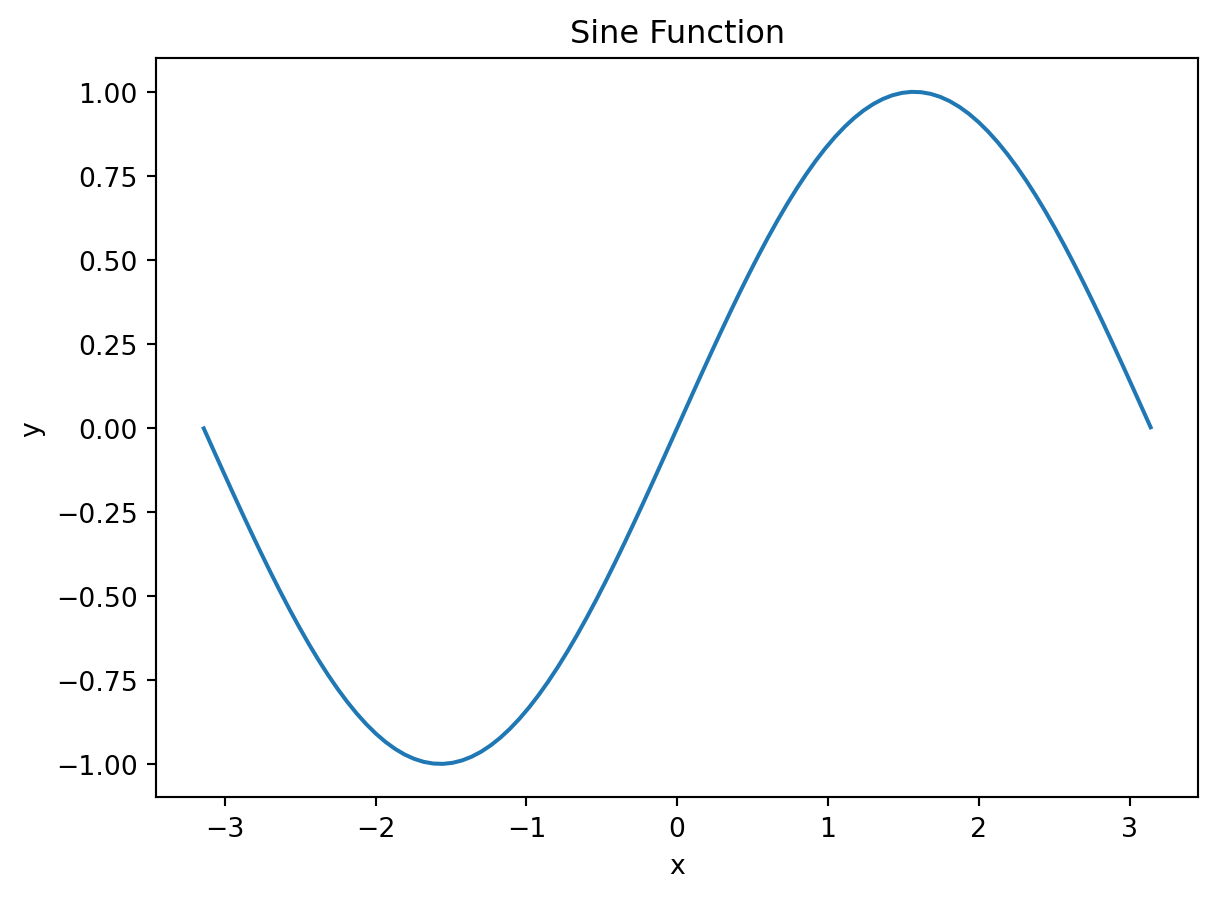
\includegraphics{taylor_files/figure-pdf/cell-2-output-1.pdf}

}

\end{figure}

\hypertarget{first-order-taylor-approximation-for-fx-at-x-0}{%
\section{First order Taylor approximation for f(x) at x =
0}\label{first-order-taylor-approximation-for-fx-at-x-0}}

\begin{Shaded}
\begin{Highlighting}[]
\NormalTok{x }\OperatorTok{=}\NormalTok{ torch.tensor([}\FloatTok{0.}\NormalTok{], requires\_grad}\OperatorTok{=}\VariableTok{True}\NormalTok{)}
\NormalTok{y }\OperatorTok{=}\NormalTok{ f(x)}
\NormalTok{approx }\OperatorTok{=}\NormalTok{ y }\OperatorTok{+}\NormalTok{ torch.autograd.grad(y, x, create\_graph}\OperatorTok{=}\VariableTok{True}\NormalTok{)[}\DecValTok{0}\NormalTok{] }\OperatorTok{*}\NormalTok{ x}
\NormalTok{x\_vals }\OperatorTok{=}\NormalTok{ torch.linspace(}\OperatorTok{{-}}\NormalTok{np.pi, np.pi, }\DecValTok{100}\NormalTok{)}
\NormalTok{y\_vals }\OperatorTok{=}\NormalTok{ f(x\_vals)}
\NormalTok{approx\_vals }\OperatorTok{=}\NormalTok{ (approx.detach() }\OperatorTok{+}\NormalTok{ torch.autograd.grad(approx, x, create\_graph}\OperatorTok{=}\VariableTok{True}\NormalTok{)[}\DecValTok{0}\NormalTok{] }\OperatorTok{*}\NormalTok{ x\_vals).detach()}
\NormalTok{plt.plot(x\_vals.numpy(), y\_vals.numpy(), label}\OperatorTok{=}\StringTok{\textquotesingle{}sin(x)\textquotesingle{}}\NormalTok{)}
\NormalTok{plt.plot(x\_vals.numpy(), approx\_vals.numpy(), label}\OperatorTok{=}\StringTok{\textquotesingle{}approx\textquotesingle{}}\NormalTok{)}
\NormalTok{plt.legend()}
\NormalTok{plt.show()}
\end{Highlighting}
\end{Shaded}

\begin{figure}[H]

{\centering 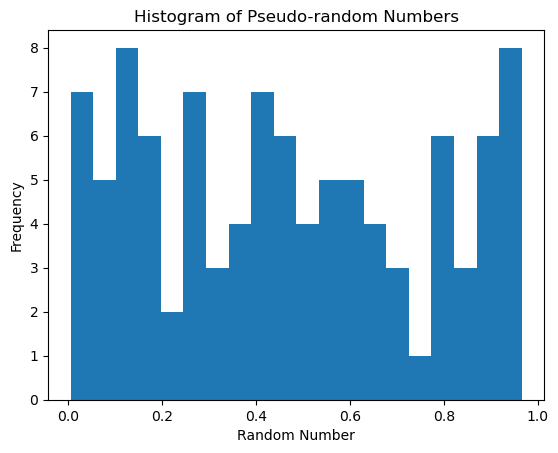
\includegraphics{taylor_files/figure-pdf/cell-3-output-1.pdf}

}

\end{figure}

\hypertarget{find-the-nth-order-taylor-approximation-for-fx-at-x-0}{%
\section{Find the nth order Taylor approximation for f(x) at x =
0}\label{find-the-nth-order-taylor-approximation-for-fx-at-x-0}}

\begin{Shaded}
\begin{Highlighting}[]
\KeywordTok{def}\NormalTok{ fact(n):}
    \ControlFlowTok{return}\NormalTok{ math.factorial(n)}

\KeywordTok{def}\NormalTok{ nth\_deriv(f, a, n):}
    \ControlFlowTok{if} \BuiltInTok{isinstance}\NormalTok{(a, (}\BuiltInTok{float}\NormalTok{, }\BuiltInTok{int}\NormalTok{)):}
\NormalTok{        a }\OperatorTok{=}\NormalTok{ torch.tensor([a], dtype}\OperatorTok{=}\NormalTok{torch.}\BuiltInTok{float}\NormalTok{, requires\_grad}\OperatorTok{=}\VariableTok{True}\NormalTok{)}
    \ControlFlowTok{else}\NormalTok{:}
\NormalTok{        a }\OperatorTok{=}\NormalTok{ a.clone().detach().requires\_grad\_(}\VariableTok{True}\NormalTok{)}
    
\NormalTok{    y }\OperatorTok{=}\NormalTok{ f(a)}
    \ControlFlowTok{for}\NormalTok{ i }\KeywordTok{in} \BuiltInTok{range}\NormalTok{(n):}
\NormalTok{        y }\OperatorTok{=}\NormalTok{ torch.autograd.grad(y, a, create\_graph}\OperatorTok{=}\VariableTok{True}\NormalTok{)[}\DecValTok{0}\NormalTok{]}
    \ControlFlowTok{return}\NormalTok{ y}



\CommentTok{\# nth degree Taylor polynomial of f(x) around x=a}
\KeywordTok{def}\NormalTok{ taylor(f, x, n):}
\NormalTok{    result }\OperatorTok{=}\NormalTok{ torch.zeros\_like(x)}
    \ControlFlowTok{for}\NormalTok{ i }\KeywordTok{in} \BuiltInTok{range}\NormalTok{(n}\OperatorTok{+}\DecValTok{1}\NormalTok{):}
\NormalTok{        result }\OperatorTok{+=}\NormalTok{ nth\_deriv(f, }\DecValTok{0}\NormalTok{, i) }\OperatorTok{/}\NormalTok{ torch.tensor(math.factorial(i), dtype}\OperatorTok{=}\NormalTok{torch.float32) }\OperatorTok{*}\NormalTok{ (x}\OperatorTok{**}\NormalTok{i)}
    \ControlFlowTok{return}\NormalTok{ result}
\NormalTok{x\_vals }\OperatorTok{=}\NormalTok{ torch.linspace(}\OperatorTok{{-}}\NormalTok{math.pi, math.pi, }\DecValTok{200}\NormalTok{)}
\NormalTok{plt.plot(x\_vals.numpy(), f(x\_vals).numpy(), label}\OperatorTok{=}\StringTok{\textquotesingle{}f(x)\textquotesingle{}}\NormalTok{, lw}\OperatorTok{=}\DecValTok{5}\NormalTok{)}
\NormalTok{plt.plot(x\_vals.numpy(), taylor(f, x\_vals, }\DecValTok{1}\NormalTok{).detach().numpy(), label}\OperatorTok{=}\StringTok{\textquotesingle{}Taylor approximation, n=1\textquotesingle{}}\NormalTok{)}
\NormalTok{plt.plot(x\_vals.numpy(), taylor(f, x\_vals, }\DecValTok{3}\NormalTok{).detach().numpy(), label}\OperatorTok{=}\StringTok{\textquotesingle{}Taylor approximation, n=3\textquotesingle{}}\NormalTok{)}
\NormalTok{plt.plot(x\_vals.numpy(), taylor(f, x\_vals, }\DecValTok{5}\NormalTok{).detach().numpy(), label}\OperatorTok{=}\StringTok{\textquotesingle{}Taylor approximation, n=5\textquotesingle{}}\NormalTok{)}
\NormalTok{plt.legend()}
\NormalTok{plt.show()}
\end{Highlighting}
\end{Shaded}

\begin{figure}[H]

{\centering 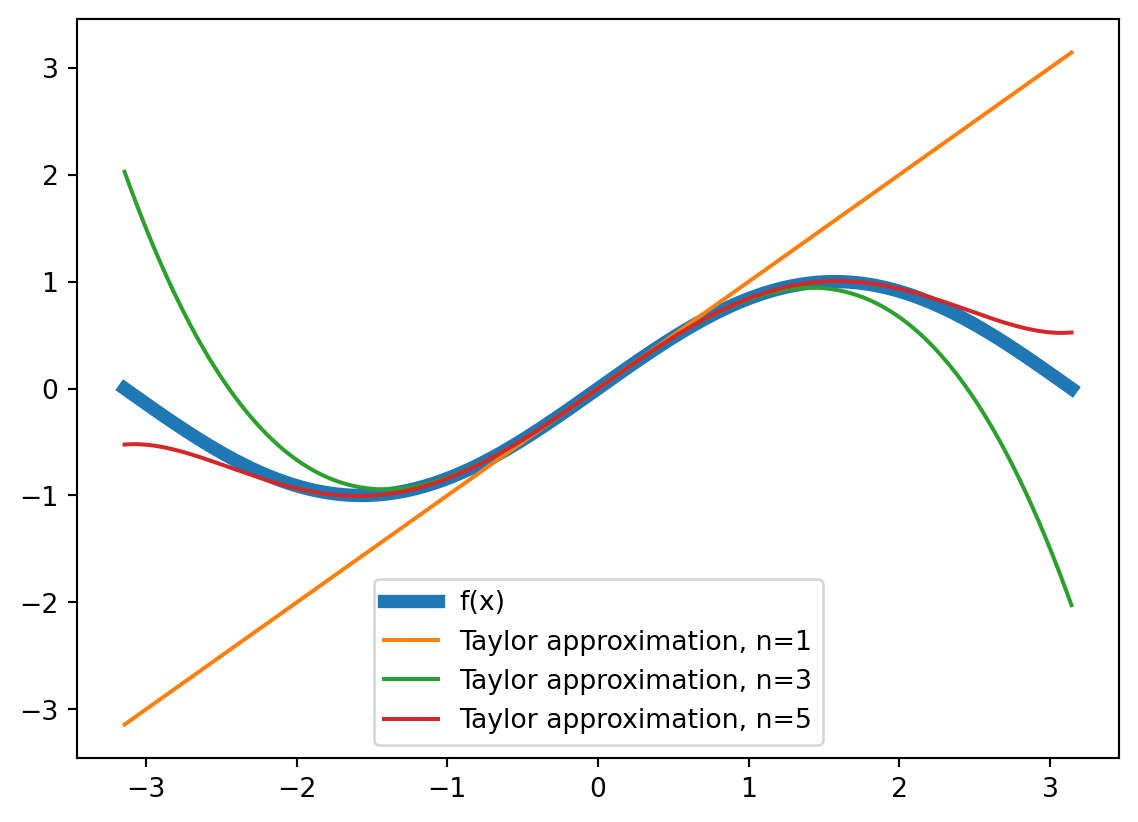
\includegraphics{taylor_files/figure-pdf/cell-4-output-1.pdf}

}

\end{figure}

\hypertarget{plot-of-the-function-gx-x2-and-its-taylor-approximations-up-to-degree-1-and-degree-2-centered-at-x0.}{%
\section{Plot of the function g(x) = x\^{}2 and its Taylor
approximations up to degree 1 and degree 2 centered at
x=0.}\label{plot-of-the-function-gx-x2-and-its-taylor-approximations-up-to-degree-1-and-degree-2-centered-at-x0.}}

\begin{Shaded}
\begin{Highlighting}[]
\NormalTok{x\_vals }\OperatorTok{=}\NormalTok{ torch.linspace(}\OperatorTok{{-}}\DecValTok{4}\NormalTok{, }\DecValTok{4}\NormalTok{, }\DecValTok{100}\NormalTok{)}

\KeywordTok{def}\NormalTok{ g(x):}
    \ControlFlowTok{return}\NormalTok{ x}\OperatorTok{**}\DecValTok{2}

\KeywordTok{def}\NormalTok{ taylor(f, x, n):}
\NormalTok{    x }\OperatorTok{=}\NormalTok{ x.unsqueeze(}\OperatorTok{{-}}\DecValTok{1}\NormalTok{)}
\NormalTok{    y }\OperatorTok{=}\NormalTok{ f(x)}
    \ControlFlowTok{for}\NormalTok{ i }\KeywordTok{in} \BuiltInTok{range}\NormalTok{(}\DecValTok{1}\NormalTok{, n}\OperatorTok{+}\DecValTok{1}\NormalTok{):}
\NormalTok{        y }\OperatorTok{+=}\NormalTok{ (x }\OperatorTok{{-}}\NormalTok{ x[}\DecValTok{0}\NormalTok{])}\OperatorTok{**}\NormalTok{i }\OperatorTok{/}\NormalTok{ torch.tensor([math.factorial(i)]).}\BuiltInTok{float}\NormalTok{() }\OperatorTok{*}\NormalTok{ f(x[}\DecValTok{0}\NormalTok{] }\OperatorTok{+} \FloatTok{0.0}\NormalTok{)}
    \ControlFlowTok{return}\NormalTok{ y}


\NormalTok{plt.plot(x\_vals.numpy(), g(x\_vals).numpy(), label}\OperatorTok{=}\StringTok{\textquotesingle{}g(x)\textquotesingle{}}\NormalTok{, lw}\OperatorTok{=}\DecValTok{5}\NormalTok{)}
\NormalTok{plt.plot(x\_vals.numpy(), taylor(g, x\_vals, }\DecValTok{1}\NormalTok{).detach().numpy(), label}\OperatorTok{=}\StringTok{\textquotesingle{}Taylor approximation, n=1\textquotesingle{}}\NormalTok{)}
\NormalTok{plt.plot(x\_vals.numpy(), taylor(g, x\_vals, }\DecValTok{3}\NormalTok{).detach().numpy(), label}\OperatorTok{=}\StringTok{\textquotesingle{}Taylor approximation, n=3\textquotesingle{}}\NormalTok{)}
\NormalTok{plt.plot(x\_vals.numpy(), taylor(g, x\_vals, }\DecValTok{5}\NormalTok{).detach().numpy(), label}\OperatorTok{=}\StringTok{\textquotesingle{}Taylor approximation, n=5\textquotesingle{}}\NormalTok{)}
\NormalTok{plt.legend()}
\NormalTok{plt.show()}
\end{Highlighting}
\end{Shaded}

\begin{figure}[H]

{\centering 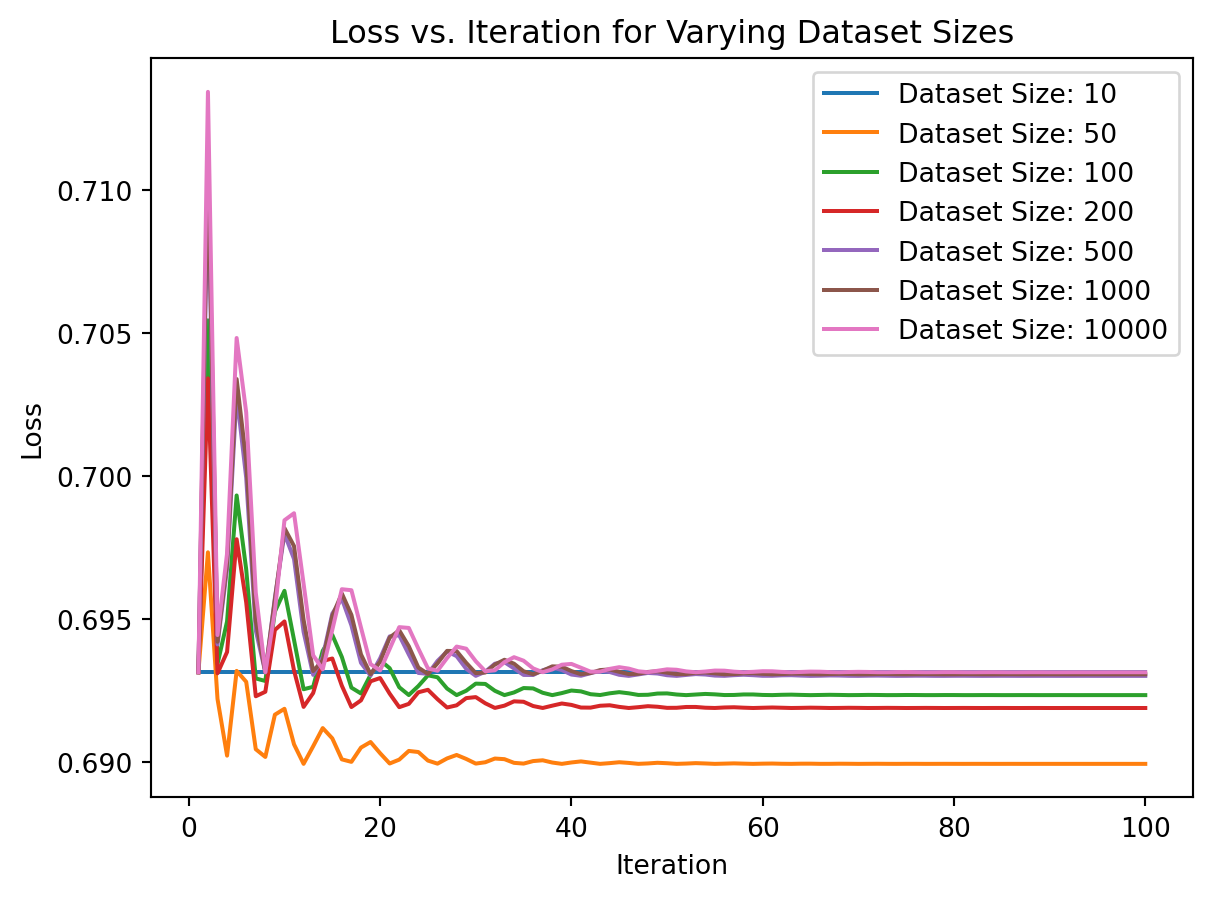
\includegraphics{taylor_files/figure-pdf/cell-5-output-1.pdf}

}

\end{figure}



\end{document}
